\documentclass[a4paper, 11pt]{article}

\voffset -0cm
\hoffset 0.0cm
\textheight 23cm
\textwidth 16cm
\topmargin 0.0cm
\oddsidemargin 0.0cm
\evensidemargin 0.0cm

\usepackage{epsfig}
\usepackage{setspace}
\usepackage{fancyheadings}
\usepackage{amsmath}
\usepackage{amssymb}
\usepackage{graphicx}
\usepackage{url}

\title{}
\author{}
\date{}

\begin{document}

\begin{center}
	\LARGE \textbf{TD6: Border Extraction and DSS Segmentation}
\end{center}

\bigskip
\par In this TP, we perform elementary geometrical analysis of digital contours using Digital Straight Segments. We assume that:
\begin{itemize}
	\item You have DGtal and DGtalSkel tools up and running (cf TP5)
	\item You have the function that construct the Gauss digitization of an Euclidean disc (as a \texttt{DigitalSet}, cf TP5)
\end{itemize}

% -------------------------------------------------------
\section*{Exercise 1 \rm Border extraction (sequel and end)}

\par The objective here is to construct the ordered sequence of pixels (either (0)- or (1)-connected) corresponding to a $(\kappa,\lambda)-$Jordan pair. The algorithm is the following:
\begin{itemize}
	\item Scan the domain to locate a first border point
	\item Given an orientation (cf Figure 1) and the last two points, check the neighbors points to decide the next border point. More precisely, starting by the first point, if it belongs to the object, it is the next one. Otherwise, "probe" the next one.
\end{itemize}

\par At each step, you'll have to "rotate" the half-masks according to the last move. You can easily check that the above algorithm generates points which are $\lambda-$adjacent to background points.

{\bf Question } Implement such border tracker and test it on the \texttt{DigitalSet} obtained by the Gauss digitization of an Euclidean disc. Note that the output of the tracker cannot be a \texttt{DigitalSet} (which is an un-ordered set of points). Instead, you could use a \texttt{vector<Point>} (don't forget the \texttt{using namespace std;}).

\begin{figure}[h]
\centering
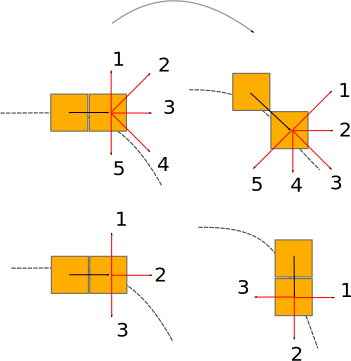
\includegraphics[width=8cm]{orientations}
\caption{Illustration of the border tracker algorithm.}
\end{figure}


% ----------------------------------------------------------------------
\section*{Exercise 2 \rm Segmentation into maximal DSS}

\par In \texttt{DGtal}, we use the DSS recognition algorithm implemented in the \texttt{ArithmeticalDSS} class. In the DGtalSkel folder (checkout the last version), you would find and example of \texttt{ArithmeticalDSS} usage. Note that the technical documentation of this class is available at \url{http://dgtal.org/doc/stable/classDGtal_1_1ArithmeticalDSSComputer.html}.

{\bf Questions:}
\begin{itemize}
	\item Have a look to the \texttt{DSSExample.cpp} file. Use \texttt{front()} and \texttt{back()} methods and return the Euclidean length of the DSS.
	\item  Customize \texttt{DSSExample.cpp} to add more points (such that the complete sequence is not a DSS anymore) and construct a decomposition of such contour into maximal DSS (cf Figure 2 for an example for the 4-connected case).
	\begin{figure}[h]
	\centering
	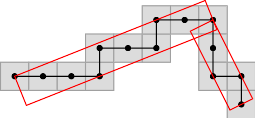
\includegraphics[width=4cm]{exampleDSS-3.png}
	\caption{Example of a 4-DSS decomposition of a small point sequence.}
	\end{figure}

	\item From the first exercise, compute the sequence defined as the border of a digital disc and compute its decomposition into maximal DSS. Display the contour and each segment to a board output and estimate the length of the contour in the meantime (sum of DSS Euclidean length).  Compare the estimated lengths to $2\pi R$ when you increase the ball radius.
\end{itemize}

\end{document}
